\begin{frame}

\frametitle{Mixture models}
\begin{itemize}
\item A mixture model is a probability distribution with density function, $f$, defined as a linear combination of density functions, $f_1, \dots f_k$, coming from other probability distributions.
\[
f(x, \blue{\pi_1}, \dots, \blue{\pi_k}, \blue{\theta_1}, \dots, \blue{\theta_k}) = \blue{\pi_1} f_1(x, \blue{\theta_1}) + \dots + \blue{\pi_k} f_k(x, \blue{\theta_k})
\]
\item Given a  sample $X$, parameters $\blue{\pi_1}, \dots, \blue{\pi_k}, \blue{\theta_1}, \dots, \blue{\theta_k}$ can be estimated using the $EM$ algorithm.
\item $EM$-algorithm needs the number of components is fixed.
\end{itemize}
\end{frame}

\begin{frame}
\frametitle{Mixture models: classifying observation}

\begin{itemize}
\item Adjusted density function:
\[
f(x) = \pi_1 \gga{f_1}(x) + \pi_2 \ggb{f_2}(x) + \pi_3 \ggc{f_3}(x) + \pi_4 \ggd{f_4}(x) + \pi_5 \gge{f_5}(x) + \pi_6 \ggf{f_6}(x)
\]
\item Any observation $x_i$ can be classified to component $j$ with maximimum
\begin{eqnarray*} \tau_{ij} &=& \frac{\pi_j f_j(x_i)}{f(x_i) } \end{eqnarray*}
\end{itemize}

\uncover<2->{%
\only<1-2>{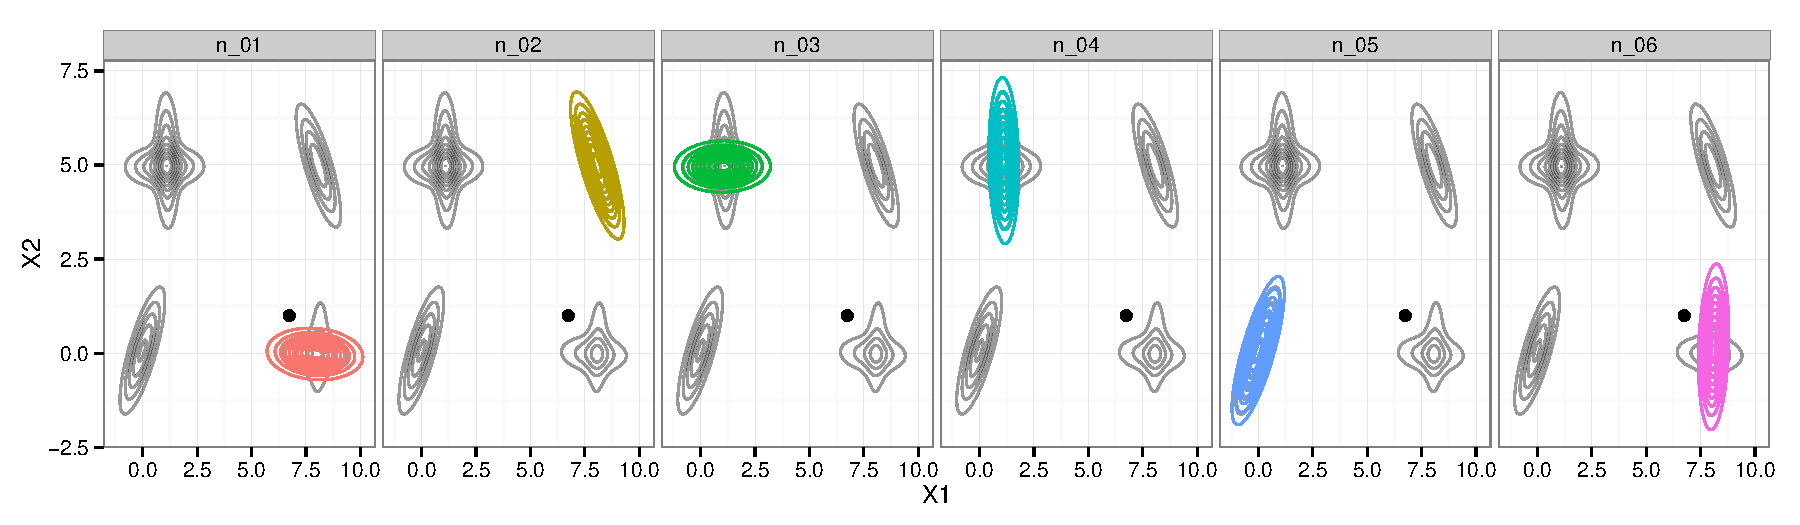
\includegraphics[width=\textwidth]{static_figures/baudry_ex4_1_all_distributions_one.pdf}}%
\only<3>{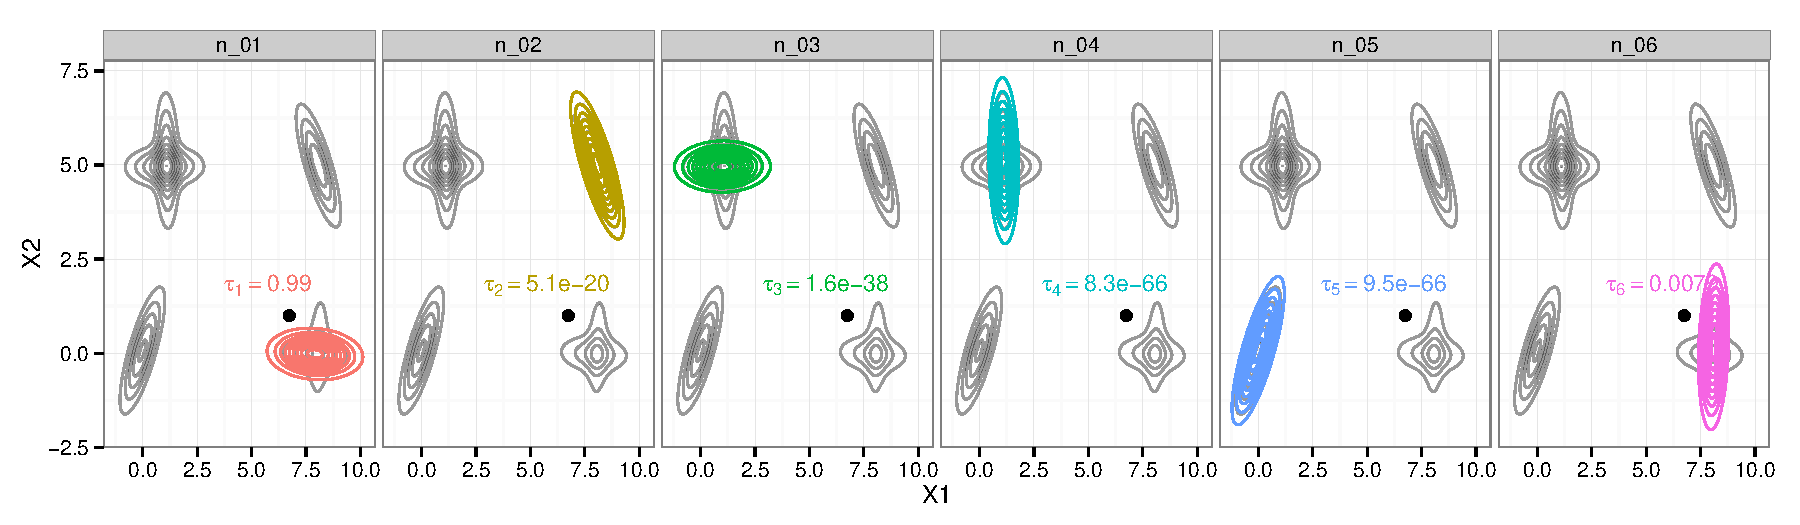
\includegraphics[width=\textwidth]{static_figures/baudry_ex4_1_all_distributions_one_tau.pdf}}}
\end{frame}

\begin{frame}
\frametitle{Mixture models: merging components}

\begin{columns}[T]
\column{0.4\textwidth}
\centering
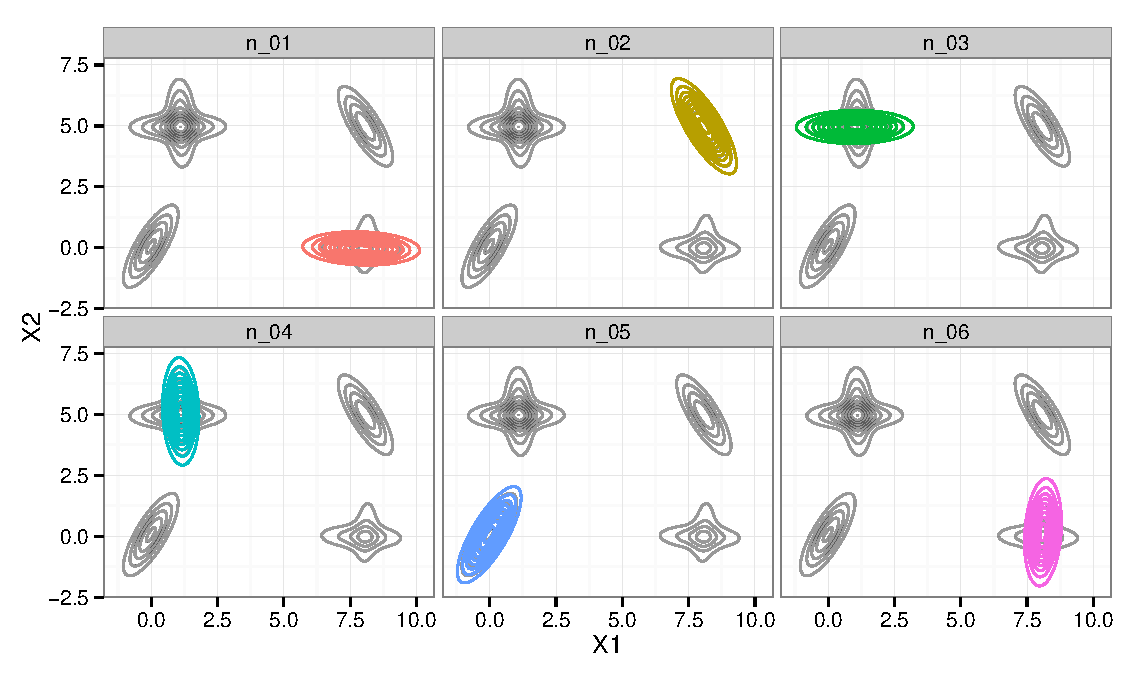
\includegraphics[width=0.9\textwidth]{static_figures/baudry_ex4_1_all_distributions.pdf}

\bigskip
\uncover<2->{%
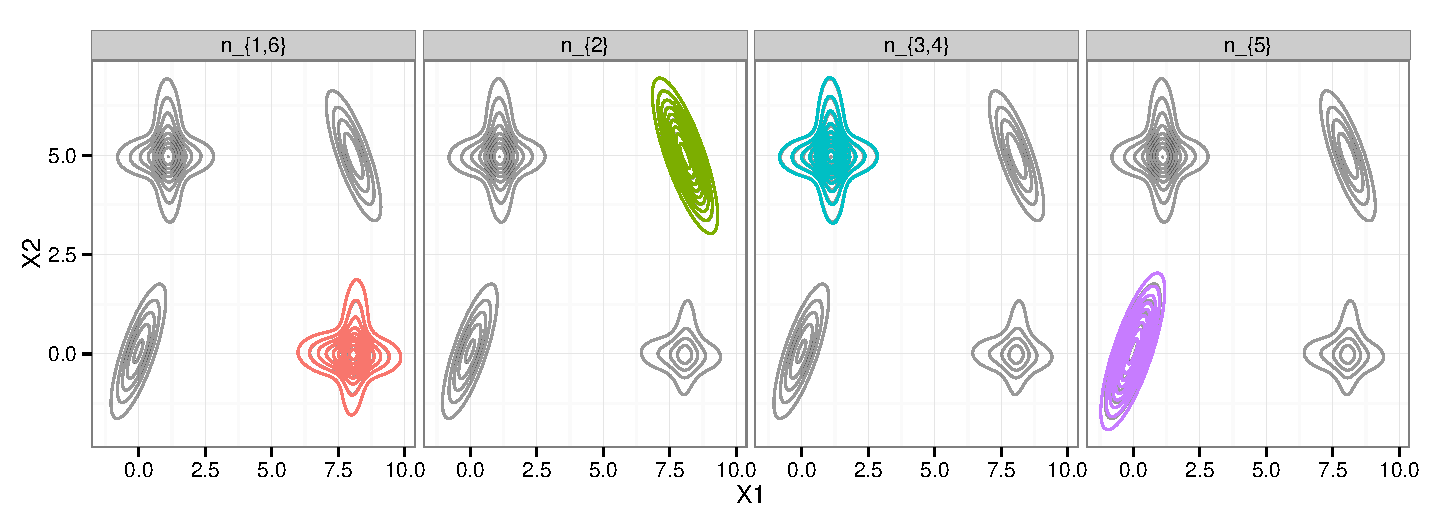
\includegraphics[width=\textwidth]{static_figures/baudry_ex4_1_all_distributions_4c.pdf}

\uncover<3->{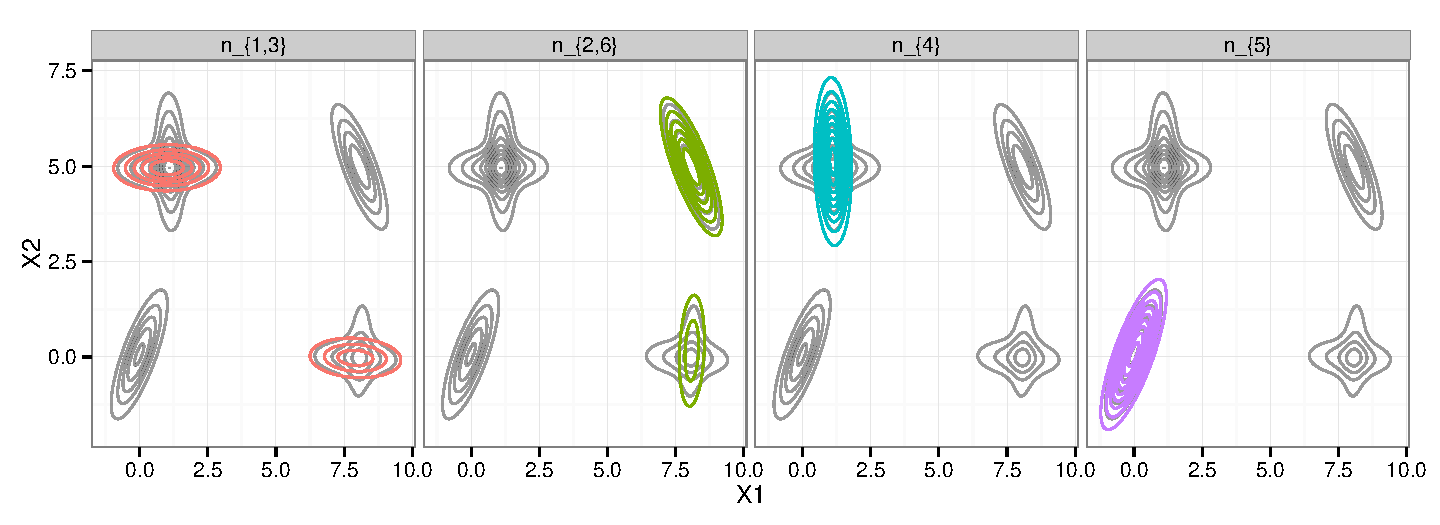
\includegraphics[width=\textwidth]{static_figures/baudry_ex4_1_all_distributions_4c_b.pdf}}
}

\column{0.6\textwidth}
\small
\begin{itemize}
\item Maybe one cluster is better explained as one mixture of components (``mixture of mixtures'')
\item<2-> From a likelihood point of view it is not possible to choose which ``mixture of mixtures'' is better.
\item<3-> Non-identificability: Both mixtures have the same likelihood.
\item<4> Different authors propose methods to merge components two by two.
\item<4> Here we focus on those methods based on posteriori probabilities which combines the components hierarchically.
\end{itemize}
\end{columns}
\end{frame}

\begin{frame}[t]
\frametitle{Mixture models: hierarchical component merging}
\begin{columns}[T]
\column{0.5\textwidth}
\small
Starting from a mixture model where each component is a cluster

\medskip

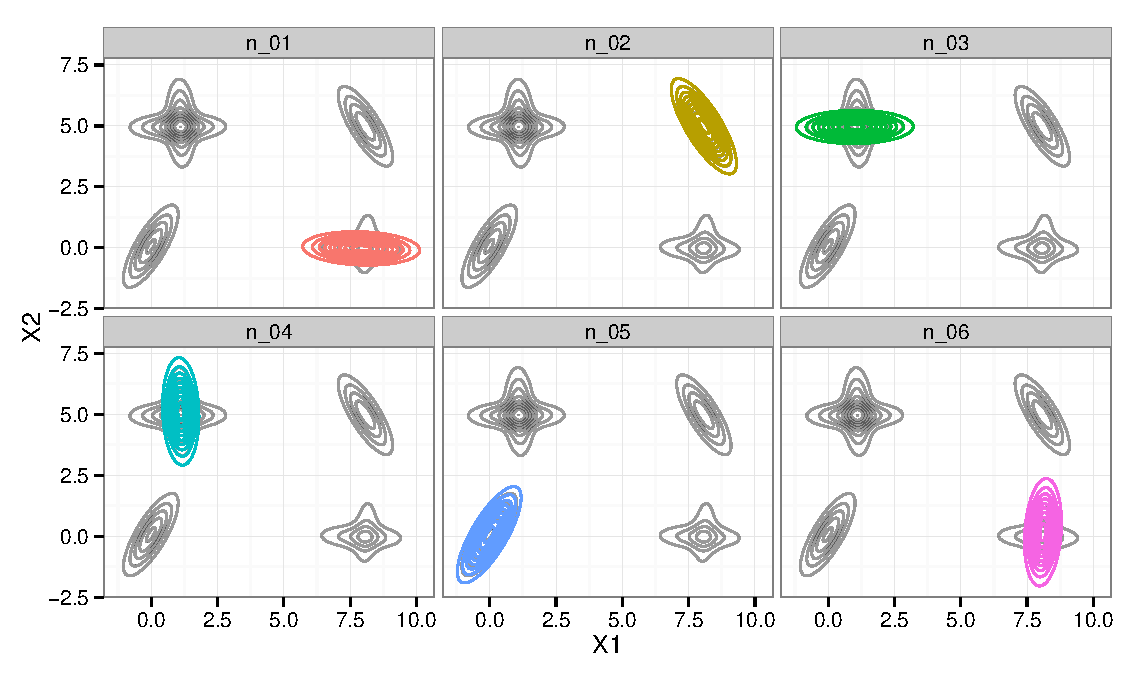
\includegraphics[width=0.9\textwidth]{static_figures/baudry_ex4_1_all_distributions.pdf}

combine sequentially the components to obtain a hierarchy over the set of components.

\pause
\column{0.5\textwidth}
\centering
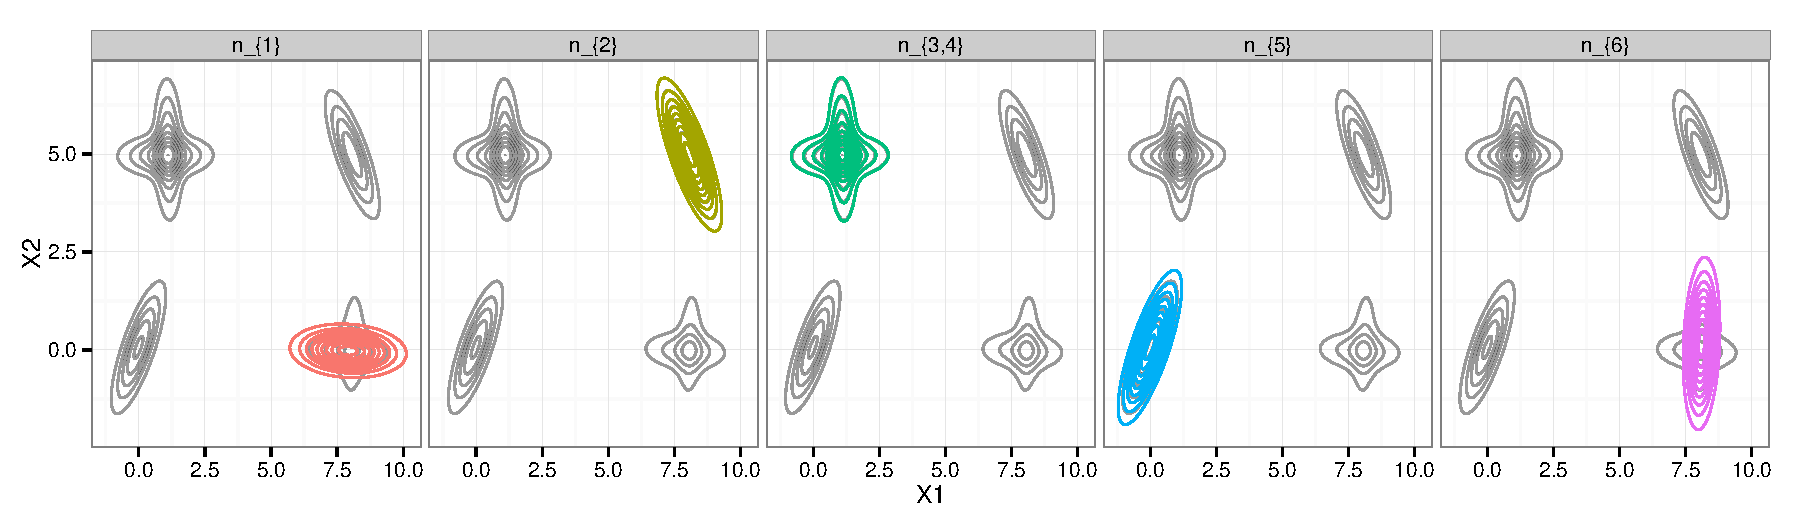
\includegraphics[height=0.2\textheight]{static_figures/baudry_ex4_1_all_distributions_5c.pdf}

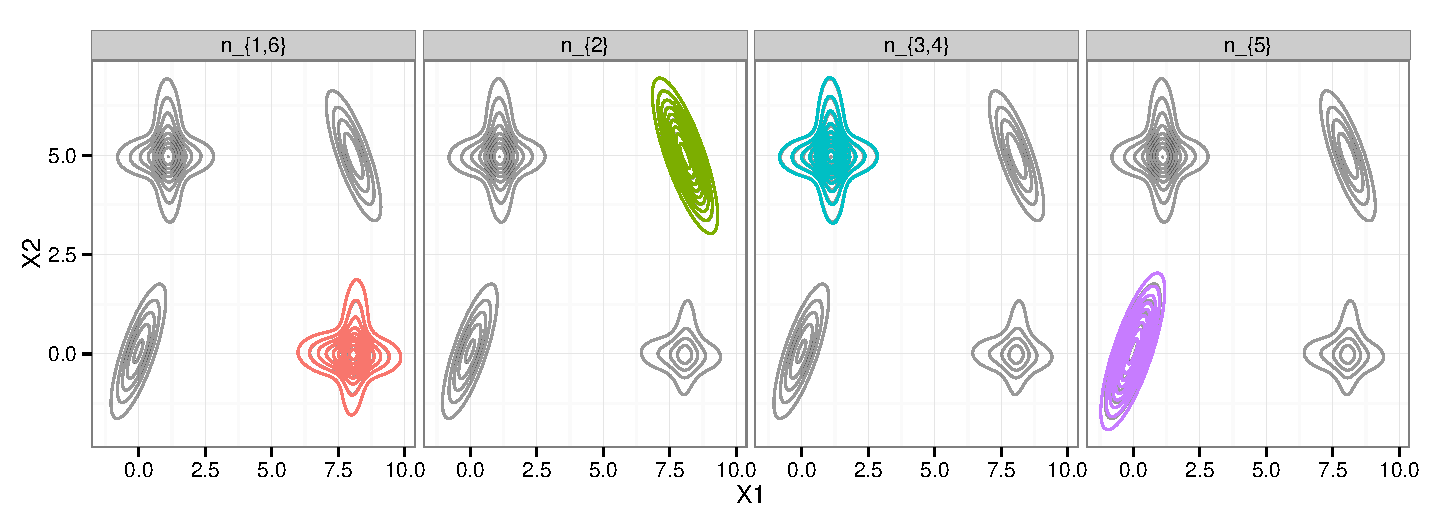
\includegraphics[height=0.2\textheight]{static_figures/baudry_ex4_1_all_distributions_4c.pdf}

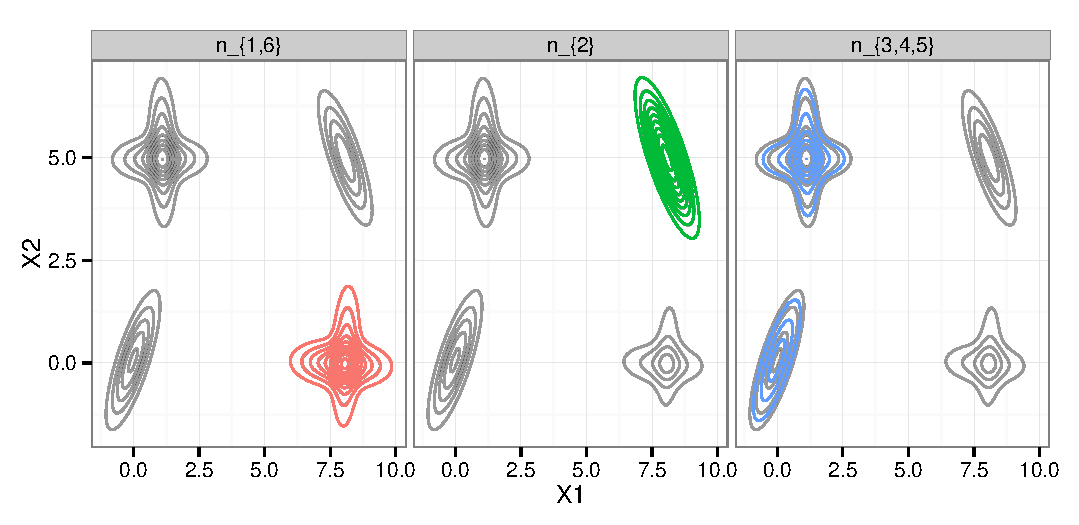
\includegraphics[height=0.2\textheight]{static_figures/baudry_ex4_1_all_distributions_3c.pdf} 

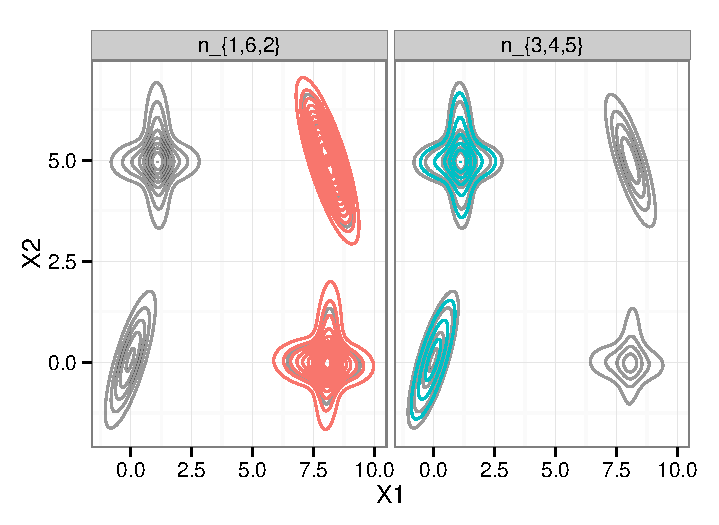
\includegraphics[height=0.2\textheight]{static_figures/baudry_ex4_1_all_distributions_2c.pdf}
\end{columns}
\end{frame}

